\documentclass[twocolumn]{article}
\usepackage{graphicx}

\begin{document}

\title{Title}
\maketitle

\section{Section 1}

Various stuff here.

\section{Section 2}

BEGIN [Tyler, Week 3]

In this section, we explore whether \_\_\_.  Figure~\ref{fig:cases}
shows \_\_\_:

\begin{figure}[h]
  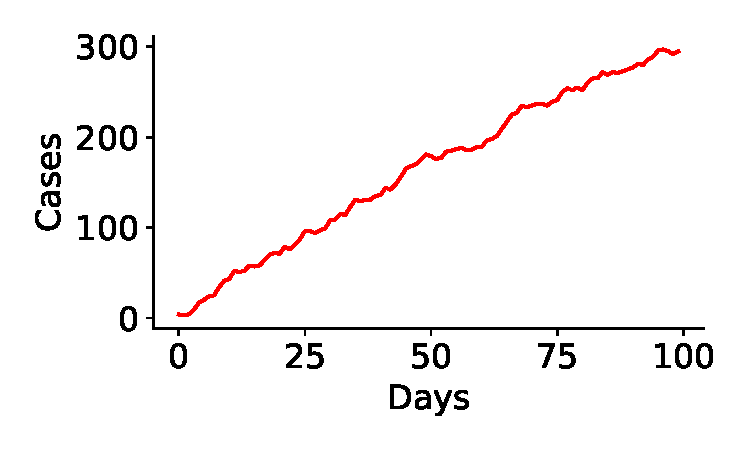
\includegraphics[width=\columnwidth]{cases.pdf}
  \caption{Cases over Time.}
  \label{fig:cases}
\end{figure}

\begin{figure}[h]
  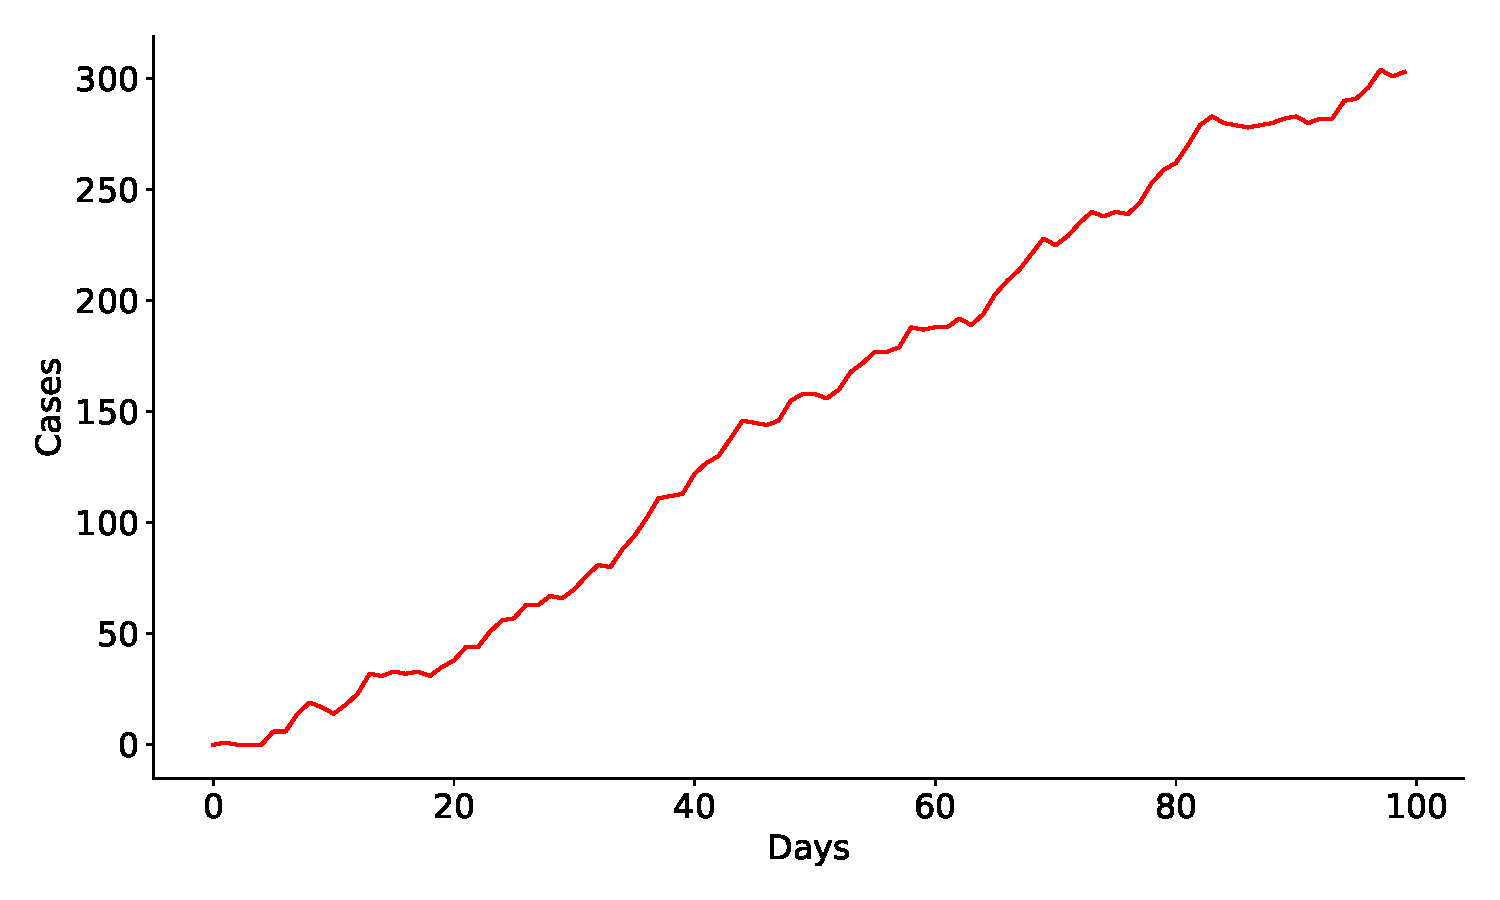
\includegraphics[width=\columnwidth]{cases2.pdf}
  \caption{Cases over Time V2.}
  \label{fig:cases2}
\end{figure}


\begin{figure*}[h]
  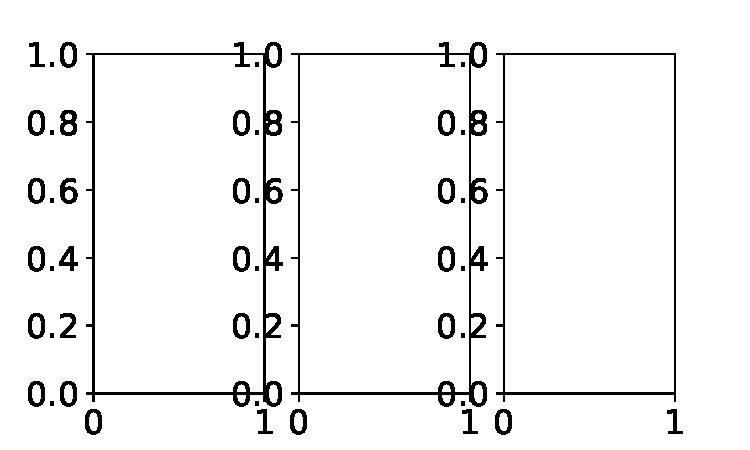
\includegraphics[width=\textwidth]{wide.pdf} % \columnwidth
  \caption{Whole page width!.}
  \label{fig:wide}
\end{figure*}

We observe that \_\_\_.  We conclude \_\_\_.

END

Other stuff.

\end{document}
